\documentclass[12pt,]{article}
\usepackage[T1]{fontenc}
\usepackage{lmodern}
\usepackage{amssymb,amsmath}
\usepackage{ifxetex,ifluatex}
\usepackage{fixltx2e} % provides \textsubscript
% use upquote if available, for straight quotes in verbatim environments
\IfFileExists{upquote.sty}{\usepackage{upquote}}{}
\ifnum 0\ifxetex 1\fi\ifluatex 1\fi=0 % if pdftex
  \usepackage[utf8]{inputenc}
\else % if luatex or xelatex
  \ifxetex
    \usepackage{mathspec}
    \usepackage{xltxtra,xunicode}
  \else
    \usepackage{fontspec}
  \fi
  \defaultfontfeatures{Mapping=tex-text,Scale=MatchLowercase}
  \newcommand{\euro}{€}
\fi
% use microtype if available
\IfFileExists{microtype.sty}{\usepackage{microtype}}{}
\usepackage[margin=1in]{geometry}
\usepackage{graphicx}
% Redefine \includegraphics so that, unless explicit options are
% given, the image width will not exceed the width of the page.
% Images get their normal width if they fit onto the page, but
% are scaled down if they would overflow the margins.
\makeatletter
\def\ScaleIfNeeded{%
  \ifdim\Gin@nat@width>\linewidth
    \linewidth
  \else
    \Gin@nat@width
  \fi
}
\makeatother
\let\Oldincludegraphics\includegraphics
{%
 \catcode`\@=11\relax%
 \gdef\includegraphics{\@ifnextchar[{\Oldincludegraphics}{\Oldincludegraphics[width=\ScaleIfNeeded]}}%
}%
\ifxetex
  \usepackage[setpagesize=false, % page size defined by xetex
              unicode=false, % unicode breaks when used with xetex
              xetex]{hyperref}
\else
  \usepackage[unicode=true]{hyperref}
\fi
\hypersetup{breaklinks=true,
            bookmarks=true,
            pdfauthor={},
            pdftitle={},
            colorlinks=true,
            citecolor=blue,
            urlcolor=blue,
            linkcolor=magenta,
            pdfborder={0 0 0}}
\urlstyle{same}  % don't use monospace font for urls
\setlength{\parindent}{0pt}
\setlength{\parskip}{6pt plus 2pt minus 1pt}
\setlength{\emergencystretch}{3em}  % prevent overfull lines
\setcounter{secnumdepth}{0}

\author{}
\date{}
\usepackage{lineno}
\linenumbers
\usepackage{setspace}
\doublespacing

\begin{document}

\normalsize


\section{Do we need detailed demographic data to forecast population
responses to climate
change?}\label{do-we-need-detailed-demographic-data-to-forecast-population-responses-to-climate-change}

\subsubsection{Andrew T. Tredennick and Peter B.
Adler}\label{andrew-t.-tredennick-and-peter-b.-adler}

\emph{Andrew T. Tredennick
(\href{mailto:atredenn@gmail.com}{\href{mailto:atredenn@gmail.com}{atredenn@gmail.com}}),
Department of Wildland Resources and the Ecology Center, Utah State
University, Logan, UT}

\emph{Peter B. Adler, Department of Wildland Resources and the Ecology
Center, Utah State University, Logan, UT}

\subsection{Abstract}\label{abstract}

\emph{Keywords}: forecasting, climate change, grassland, integral
projection model

\subsection{Introduction}\label{introduction}

Population models are important tools for predicting the impacts of
environmental change on species. But reconciling the scales at which
population models are parameterized and the scales at which
environmental changes play out remains a challenge (Freckleton et al.
2011, Queenborough et al. 2011). The major hurdle is that most
population models, at least for plant species, are built using data from
small, localized plots because parameterizing traditional population
models requires tracking the fates of individuals. These models are
difficult to scale up from the micro to meso-scales because the fitted
parameters do not fully represent the spatial variation present at
scales beyond that at which the data are collected (Sæther et al. 2007).
Thus, our ability to use population models to predict the consequences
of climate change is limited when we rely on individual-level data.

In contrast to individual-level data, population-level data arising from
large-scale census efforts

Recently, Freckleton et al. (2011), building on work by Taylor and
Hastings (2004), have proposed density-structured population models that
focus on the transition of populations among discrete states, rather
than the traditional approach of modeling the transitions of
individuals. Such an approach could be extremely valuable because the
data needed to parameterize density-structured population models is much
easier, and less costly, to collect.

For example, using a density-structured approach, one could build a
population model using a time series of annual plot-based censuses of
species percent cover. However, a major assumption of the
density-structured approach is that the aggregate dynamics of the
population observed at coarse spatial resolution faithfully represent,
and correspond to, the fates of individual plants. In other words, using
a density-structured approach requires a leap of faith that important
covariates (e.g., climate variables) at the level of the individual are
captured adequately at the population level. If we seek to forecast the
impacts of climate change on plant populations, then clearly this
assumption requires testing.

\subsection{Materials and Methods}\label{materials-and-methods}

\subsubsection{Study site and data}\label{study-site-and-data}

Our demographic data comes from the Fort Keogh Livestock and Range
Research Laboratory in eastern Montana's northern mixed prairie near
Miles City, Montana, USA (46 deg. 19' N, 105 deg 48' W). The dataset is
freely available on Ecological Archives (Anderson et al. 2011), and
interested readers should refer to the metadata therin for a complete
description. The site is about 800 m above sea level and mean annual
precipitation (1878-2009) is 334 mm, with most annual precipitaion
falling from April through September (76). The site is grass dominated
and, for the purposes of our study, we focus on the four most abundant
graminoid species: \emph{Bouteloua gracilis} (BOGR),
\emph{Hesperostipa comata} (HECO), \emph{Pascopyrum smithii} (PASM), and
\emph{Poa secunda} (POSE).

From 1932 to 1945 individual plants were identified and mapped annualy
in 44 1-m2 quadrats using a pantograph. The quadrats were distributed in
six pastures, each assigned a grazing treatment of light (1.24 ha/animal
unit month), moderate (0.92 ha/aum), and heavy (0.76 ha/aum) stocking
rates (two pastures per treatment). In this analysis we account for
potential differences among the grazing treatments, but do not focus on
grazing$\times$climate interactions. The annual maps of the quadrats
were digitized and the fates of individual plants tracked and extracted
using a computer program. Daily climate data, which we aggregated into
climate variables of interest, are available for the duration of the
data collection period (1932 - 1945) from the Miles City airport, Wiley
Field, 9 km from the study site.

In this paper, we model populations based on two levels of data:
individual and quadrat. The individual data is the ``raw'' data. For the
quadrat level we data we simply sum individual areal cover for each
quadrat by species. This is equivalent to a perfect census of quadrat
percent cover, so we do not need to consider measurement error. Based on
these two datasets we can compare population models built using
individual level data and aggregated quadrat level data.

\subsubsection{Stastical models of vital
rates}\label{stastical-models-of-vital-rates}

At both levels of inference (individual and quadrat), the building
blocks of our population models are vital rate regressions. For
individual level data we fit models for survival, growth, and
recruitment of new individuals for each species. At the quadrat level we
fit analagous models of extinction probability, percent cover
increase/decrease, and quadrat colonization for each species. We
describe the statistical models seprately since fitting the models
required different approaches at the individual and quadrat levels. All
models contain four climate covariate that we chose \emph{a priori}:
fall through spring precipitation at \emph{t}-1 and \emph{t}-2 (ppt1 and
ppt2, respectively) and mean spring temperature at \emph{t}-1 and
\emph{t}-2 (TmeanSpr1 and TmeanSpr2, respectively), where \emph{t} is
the observation year.

We fit all models using a hierarchical Bayesian approach, which we
describe in more detail below. However, for each vital rate statistical
model we also define the likelihood model we use. For the likelihood
models, Y is always the relevant vector of observations (e.g., whether a
genet survived {[}1{]} or not {[}0{]} from year $t$ to $t+1$).

\paragraph{Vital rate models: individual
level}\label{vital-rate-models-individual-level}

We used logistic regression to model survival probability ($S$) of genet
$i$ from species $j$ in quadrat group $Q$ from time $t$ to $t+1$:

\begin{align}
\text{logit}(S_{ijQ,t}) &= \gamma^{S}_{j,t} + \phi^{S}_{jQ} + \beta^{S}_{j,t}x_{ij,t} + \omega^{S}_{j}w_{ij,t} + \theta^{S}_{jk}C_{k,t} + \varepsilon^{S}_{t} \\
Y^{S}_{ijQ,t} &\sim \text{Bernoulli}(S_{ijQ,t})
\end{align}

where $x_{ij,t}$ is the log of genet size, $\gamma^{S}_{j,t}$ is a
year-specific intercept, $\beta^{S}_{j,t}$ is the year-specific slope
parameter for size, $\phi^{S}_{jQ}$ is the random effect of quadrat
group location, and $\theta^{S}_{k}$ is the fixed parameter for the
effect of the $k$th climate covariate at time $t$ ($C_{k,t}$). We
include density-dependence by estimating the effect of crowding on the
focal individual by other individuals of the same species. $\omega$ is
the effect of crowding and $w_{t,Q}$ is the crowding experienced by the
focal individual at time $t$ in quadrat group $Q$.

We modeled growth as gaussian process describing genet size at time
$t+1$ as a function of size at $t$ and climate covariates:

\begin{align}
x_{ijQ,t+1} &= \gamma^{G}_{j,t} + \phi^{G}_{jQ} + \beta^{G}_{j,t}x_{ij,t} + \omega^{G}_{j}w_{ij,t} + \theta^{G}_{jk}C_{k,t} \\
Y^{G}_{ijQ,t} &\sim \text{Normal}(x_{ijQ,t+1}, \sigma_{j})
\end{align}

where $x$ is log genet size and all other paramters are as described for
the survival regression.

Our data allows us to track new recruits, but we cannot assign a
specific parent to new genets. So, for recruitment, we work at the
quadrat level and model the number of new individuals of species $j$ in
quadrat $q$ recruiting at time $t+1$ as a function of quadrat
``effective cover'' ($A'$) in the previous year ($t$). Effective cover
is a mixture of observed cover ($A$) in the focal quadrat ($q$) and the
mean cover across the entire group ($\bar{A}$) of $Q$ quadrats in which
$q$ is located:

\begin{equation}
A'_{jq,t} = p_{j}A_{jq,t} + (1-p_{j})\bar{A}_{jQ,t}
\end{equation}

where $p$ is a mixing fraction between 0 and 1 that is estimated within
the model.

We assume the number of individuals, $Y^{R}$, recruiting at time $t+1$
follows a negative binomial distribution:

\begin{equation}
Y^{R}_{jq,t+1} \sim \text{NegBin}(\lambda_{jq,t+1},\zeta)
\end{equation}

where $\lambda$ is the mean intensity and $\zeta$ is the size parameter.
We define $\lambda$ as:

\begin{equation}
\lambda_{jq,t+1} = A'_{jq,t}e^{(\gamma^{R}_{j,t} + \phi^{R}_{jQ} + \theta^{R}_{jk}C_{k,t} + \omega^{R}\sqrt{A'_{q,t}})}
\end{equation}

where $A'$ is effective cover ($\text{cm}^2$) of species $j$ in quadrat
$q$ and all other terms are as in the survival and growth regressions.

\paragraph{Vital rate models: quadrat
level}\label{vital-rate-models-quadrat-level}

At the quadrat level we defined three vital rates:

\begin{enumerate}
\def\labelenumi{\arabic{enumi}.}
\itemsep1pt\parskip0pt\parsep0pt
\item
  Probability of extirpation ($S$): the probability that, for a given
  species, a particular quadrat will go from non-zero cover at time $t$
  to zero cover at time $t+1$.
\item
  Cover change ($G$): the change in percent cover from time $t$ to $t+1$
  for a given species within a particular quadrat.
\item
  Probability of colonization ($R$): the probability that, for a give
  species, a particular quadrat will go from zero cover at time $t$ to
  non-zero cover at time $t+1$.
\end{enumerate}

We retain the abbreviations $S$, $G$, and $R$ from the analagous
processes at the individual level. The vital rate models at the quadrat
level are all based on quadrat proportional cover. Also, at the quadrat
level we do not need to explicitly include a density dependent term.
Since we are modeling proportional cover, we essentially get
density-dependence for ``free'' when proportional cover is included as a
covariate. That is, density-dependence emerges because quadrats with low
cover gerenally increase in cover whereas quadrats with high cover
generally decrease in cover.

We modeled the probability of extirpation of species $j$ in quadrat $q$
from time $t$ to $t+1$ as:

\begin{align}
\text{logit}(S_{jq,t}) &= \gamma^{S}_{j} + \phi^{S}_{jQ} + \beta^{S}_{j}x_{jq,t} + \theta^{S}_{jk}C_{k,t} \\
Y^{S}_{jq,t} &\sim \text{Bernoulli}(S_{jq,t})
\end{align}

where all parameters are as in Eq. 1 except that $x$ is now quadrat
proportional cover. Note, however, that we do not include year random
effects on the intercept $\gamma$ or the slope term $\beta$ for quadrat
proportional cover. The quadrat data is inherently more sparse than the
individual data from which it is aggregated, and this is especially
evident when modeling rare events like extirpation and colonization.
Thus, when we tried to fit random year effects, those terms did not
converge.

We modeled quadrat cover change ($G$) from time $t$ to $t+1$ as:

\begin{equation}
\text{logit}(x_{jq,t+1}) = \gamma^{G}_{j,t} + \phi^{G}_{jQ} + \beta^{G}_{j,t}x_{jq,t} + \theta^{S}_{jk}C_{k,t}
\end{equation}

where, in this case, we do include random year effects on the intercept
$\gamma$ and the slope term $\beta$. For cover change we had enough data
for those terms to converge. Note that our model for quadrat cover
change uses a logit transformation to link the expected cover at $t+1$
($x_{jq,t}$) to the linear predictors. We do so because during model
fitting we use a beta likelihood since the data, proportional cover, is
beta distributed. The beta likelihood requires shape ($\rho$) and rate
($\eta$) parameters that can be caclulated using moment-matching:

\begin{align}
\rho_{jq,t+1} &= x_{jq,t+1}\tau_{j} \\
\eta_{jq,t+1} &= (1-x_{jq,t+1})\tau_{j}
\end{align}

with likelihood:

\begin{equation}
Y^{G}_{jq,t+1} \sim \text{Beta}(\rho_{jq,t+1}, \eta_{jq,t+1}).
\end{equation}

Finally, we modeled probability of colonization in quadrat $q$ by
species $j$ from time $t$ to $t+1$ as:

\begin{align}
\text{logit}(R_{jq,t}) &= \gamma^{R}_{j} + \phi^{R}_{jQ} + \theta^{R}_{jk}C_{k,t} \\
Y^{R}_{jq,t} &\sim \text{Bernoulli}(R_{jq,t}).
\end{align}

\subsubsection{Model fitting}\label{model-fitting}

Our Bayesian approach to fitting the vital rate models required choosing
appropriate priors for unknown parameters and deciding which, if any, of
those prior should be hierarchical. We decided to fit models where all
terms except climate covariates were fit by species, while the climate
covariates were fit heierarchically where species-specific coefficients
were drawn from a shared `global' coefficient distribution. We did so
for two reasons: (1) the four focal species are all perrennial grasses
that we expect to respond similarly to climate covariates, and (2)
convergence of climate effects at the quadrat level was much easier to
achieve when we modeled these terms hierarchically, allowing them to
``share'' statistical strenght via partial pooling (Gelman and Hill
2007). So, climate effects were modeled as:

\begin{align}
\theta_{jk} &\sim \text{Normal}(\bar{\theta_{k}}, \sigma_{k}) \\
\bar{\theta_{k}} &\sim \text{Normal}(0, 1e-6)
\end{align}

We used uninformative priors for all unknown parameters, specifically:

\begin{align}
\boldsymbol{\gamma, \beta} &\sim \text{Normal}(0, 1e^{-6}) \\
\boldsymbol{\phi} &\sim \text{Normal}(0, \boldsymbol{\sigma_{\phi}}) \\
\boldsymbol{\sigma_{\phi}} &\sim e^{(\text{Gamma}(2, 0.5))} \\
\boldsymbol{\sigma_{\theta}, \sigma_{\gamma}, \sigma_{\beta}, \tau, \zeta} &\sim \text{Gamma}(0.001, 0.001)
\end{align}

All of our analyses (model fitting and simulating) were conducted in R
(Team 2013). We used the MCMC sampler in JAGS (Plummer 2003) to estimate
the posterior distributions of model parameters and the package `r2jags'
(Su and Yajima 2012) to connect R to JAGS. We obtained posterior
distributions for all model parameters from three parallel MCMC chains
run for 50,000 iterations, after discarding an initial 50,000
iterations. We assessed convergence visually and using the Gelman and
Rubin (1992) diagnostic in the R package `coda' (Plummer et al. 2006).
Scale reduction factors for all parameters were less than 1.02,
indicating convergence. For the purposes of introducing stochasticity in
our population models, we saved the final 1,000 iterations from each
chain for all parameters to be used as randomly drawn values during
population simulation.

\subsubsection{Population models}\label{population-models}

With the posterior distribution of the vital rate statistical models in
hand, it is straightforward to simulate the population models.

\subsection{Results}\label{results}

We assessed the statistical importance of the climate covariates
included the final vital rate regressions by comparing the residual
deviance of models with climate covariates and temporal random effects,
climate covariates only, and temporal random effects only. When a model
includes climate covariates, this comparison shows the relative
contribution of the climate covariates in explaining the total
interannual variability (Adler et al. 2012).

\begin{figure}[htbp]
\centering
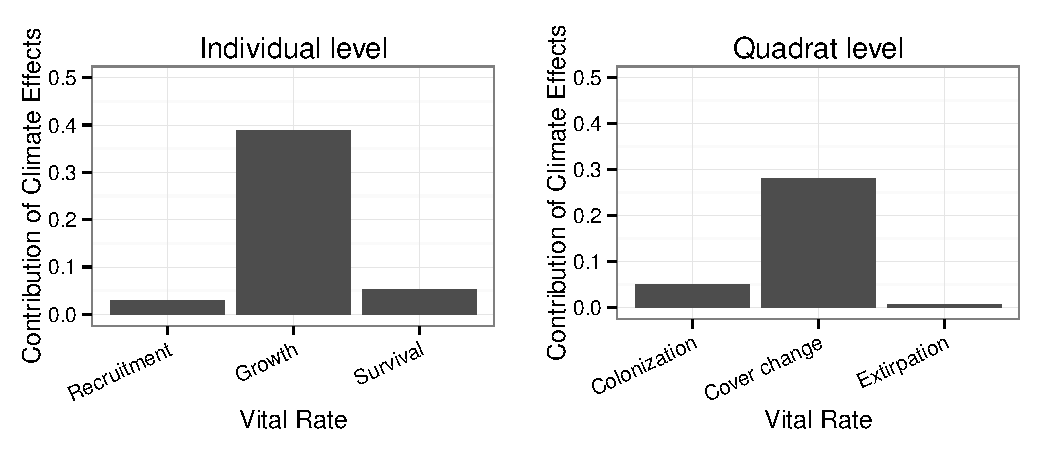
\includegraphics{components/figure/manuscript-figure_1.pdf}
\caption{The proportion of interannual variability in vital rates
explained by the climate covariates. The contribution for growth is
defined as: (Climate model - Constant Model)/(Full model - Constant
model). The contribution for survival and colonization, where we could
not estimate a full model with year random effects at the quadrat level,
is defined as: (Constant Model - Climate Model)/Constant Model.}
\end{figure}

\begin{figure}[htbp]
\centering
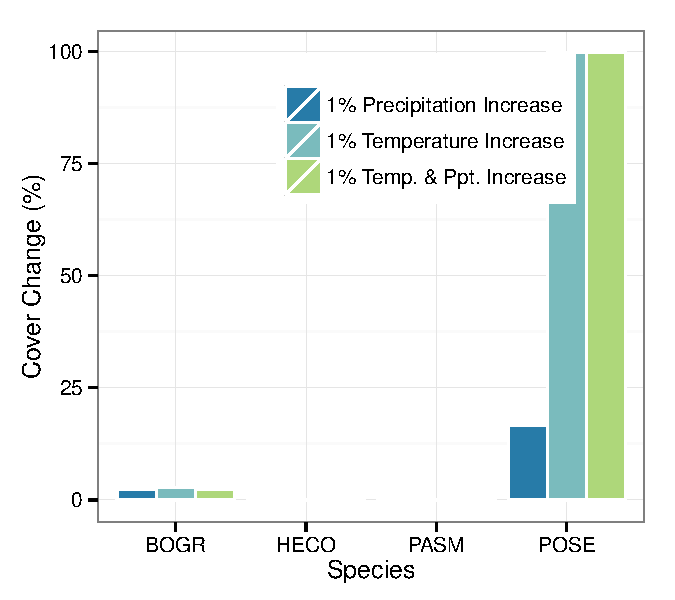
\includegraphics{components/figure/manuscript-figure_2.pdf}
\caption{Posterior means (vertical ticks), 75\% credible intervals
(heavy lines), and 95\% credible intervals (light lines) of climate
effects on growth at both levels of inferences. The dashed vertical line
is at 0, indicating no effect. Horizontal line at 0 indicates perfect
agreement between mean observed cover in that year and the model
predictions.}
\end{figure}

\begin{figure}[htbp]
\centering
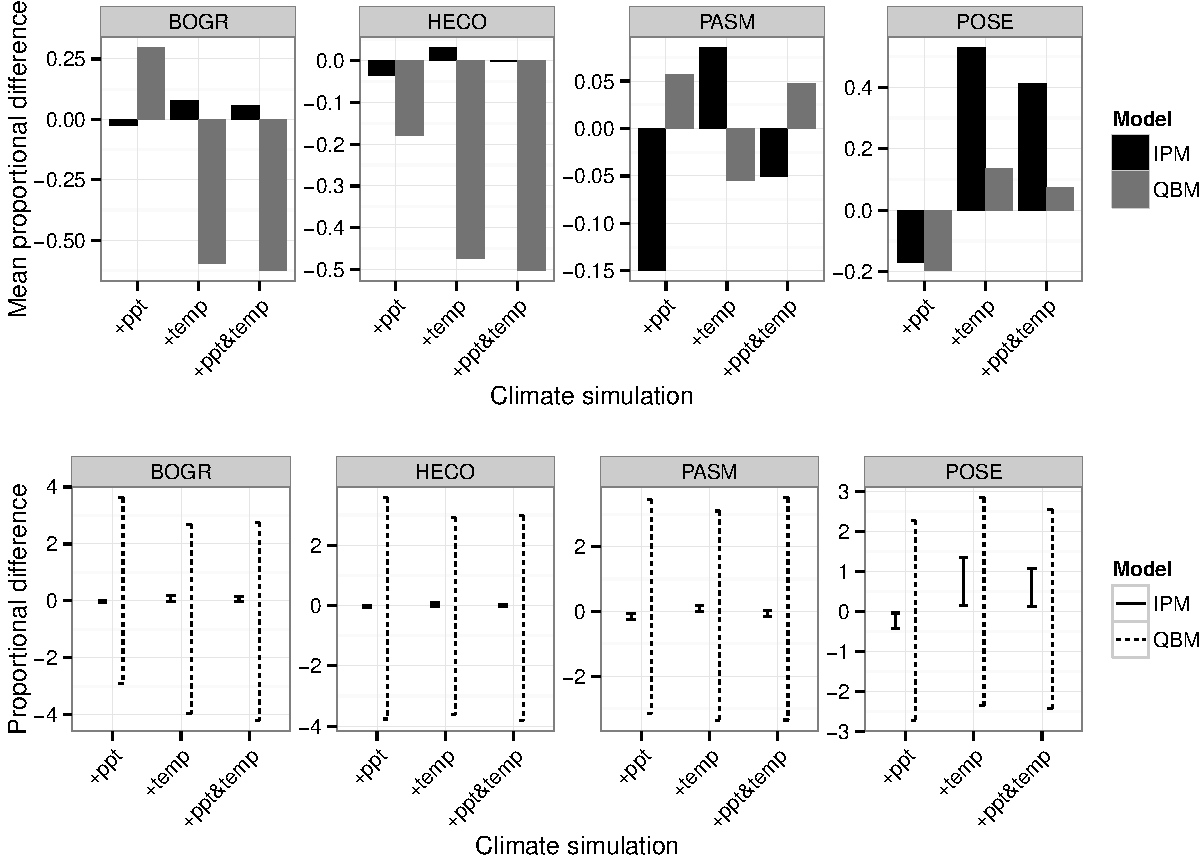
\includegraphics{components/figure/manuscript-figure_3.pdf}
\caption{Boxplots of model residuals for one-step-ahead forecasts at
each observation year. Each one-step forecast was simulated
\texttt{r nSims} times. Note that the y-axes vary across panels. The
light blue line shows the difference between the observed-year percent
cover and the average cover observed across all years. The models tend
to underpredict and perform poorly when observed cover in a given year
is a large deviant from the mean.}
\end{figure}

\subsection{References}\label{references}

Adler, P. B., H. J. Dalgleish, and S. P. Ellner. 2012. Forecasting plant
community impacts of climate variability and change: when do competitive
interactions matter? Journal of Ecology 100:478--487.

Anderson, J., L. Vermeire, and P. B. Adler. 2011. Fourteen years of
mapped, permanent quadrats in a northern mixed prairie, USA. Ecology
92:1703.

Freckleton, R. P., W. J. Sutherland, A. R. Watkinson, and S. A.
Queenborough. 2011. Density-structured models for plant population
dynamics. American Naturalist 177:1--17.

Gelman, A., and J. Hill. 2007. Data analysis using regression and
multilevel/hierarchical models. Page xxii, 625p.

Gelman, A., and D. B. Rubin. 1992. Inference from Iterative Simulation
Using Multiple Sequences.

Plummer, M. 2003. JAGS: A Program for Analysis of Bayesian Graphical
Models Using Gibbs Sampling. Pages 20--22 \emph{in} Proceedings of the
3rd international workshop on distributed statistical computing (dSC
2003). march.

Plummer, M., N. Best, K. Cowles, and K. Vines. 2006. CODA: Convergence
Diagnosis and Output Analysis for MCMC. R News 6:7--11.

Queenborough, S. A., K. M. Burnet, W. J. Sutherland, A. R. Watkinson,
and R. P. Freckleton. 2011. From meso- to macroscale population
dynamics: A new density-structured approach. Methods in Ecology and
Evolution 2:289--302.

Su, Y., and M. Yajima. 2012. R2jags: A Package for Running jags from R.
http://CRAN. R-project. org/package= R2jags.

Sæther, B. E., S. Engen, V. Grøtan, W. Fiedler, E. Matthysen, M. E.
Visser, J. Wright, A. P. Møller, F. Adriaensen, H. {Van Balen}, D.
Balmer, M. C. Mainwaring, R. H. McCleery, M. Pampus, and W. Winkel.
2007. The extended Moran effect and large-scale synchronous fluctuations
in the size of great tit and blue tit populations. Journal of Animal
Ecology 76:315--325.

Taylor, C. M., and A. Hastings. 2004. Finding optimal control strategies
for invasive species: a density-structured model for Spartina
alterniflora. Journal of Applied Ecology 41:1049--1057.

Team, R. 2013. R Development Core Team. R: A Language and Environment
for Statistical Computing.

\end{document}
